\section{Conception préliminaire}

\subsection{Diagramme de classe}

	Le diagramme présent sur la figure \ref{diagrammeClasse} permet de représenter les différentes activités et classes utilisées dans l'application. 

\begin{sidewaysfigure}
	\includegraphics[scale=0.6]{images/diagrammeClasse.png}
	\caption{Diagramme de classe}
	\label{diagrammeClasse}
\end{sidewaysfigure}

\subsection{Diagramme de navigation}
	
	Le diagramme présent sur la figure \ref{diagrammeNavigation} permet de représenter les transitions entre chaque activité de l'application. 

\begin{figure}[!h]
	\begin{center}
	
	   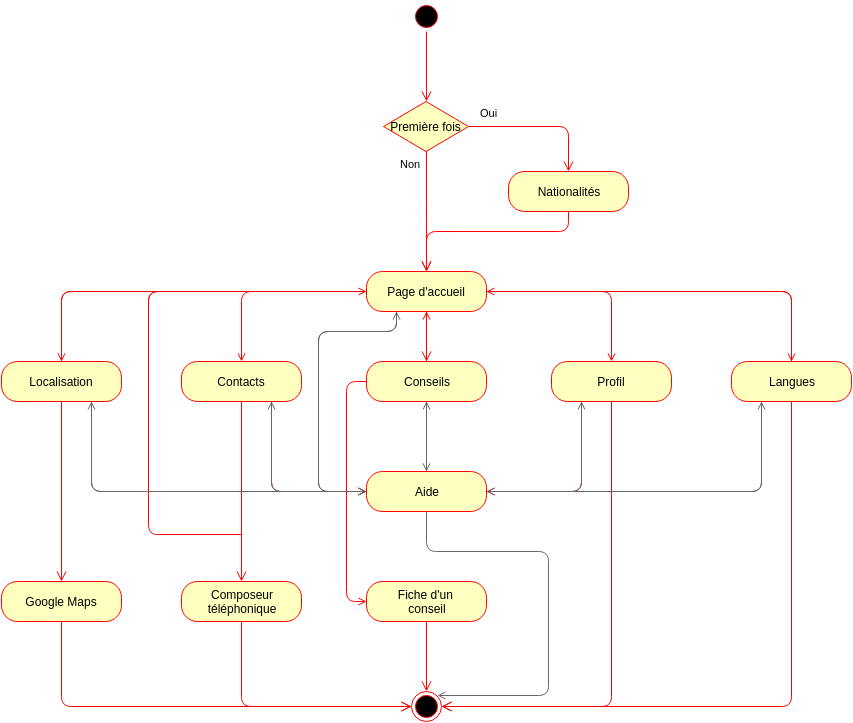
\includegraphics[scale=0.6]{images/navigation.png}
	   \caption{Diagramme de navigation}
	   \label{diagrammeNavigation} 	
	\end{center}
\end{figure}

\section{Conception détaillée}

\subsection{Package JAVA fr.touriste.gendarme.pao.gendarme}
	
\subsubsection{MainActivity}
	
	Cette activité représente l'accueil de l'application. Celle-ci permet à l'utilisateur d'accéder aux différentes fonctionnalités à savoir la localisation de services, la liste de contacts, la liste des conseils, le profil et le choix de la langue. Un raccourci permettant d'appeler les urgences (112) à aussi été placé directement sur l'accueil.
	
	On commence par initialiser la barre de navigation générale de l'application qui sera ensuite disponible à partir de n'importe quelle activité. On construit les différents boutons qui seront présents dans cette dernière à savoir celui permettant d'afficher l'aide ainsi que celui permettant d'ouvrir le menu drawer.
	\\
	
	Si la géolocalisation n'est pas activée l'application demande à l'utilisateur de l'activer dans le but d'accéder à l'apllication et de profiter pleinement de toutes les fonctionnalités disponibles. Ainsi le touriste est automatiquement redirigé dans les options et celui-ci aura le choix d'activer ou non la géolocalisation.
	
\subsubsection{ProfileActivity}
	
	Cette activité permet d'accéder au profil de l'utilisateur. Celui-ci pourra renseigner ses informations personnelles, une photo de profil ainsi que ses remarques médicales.
	\\
	
	On commence par mettre en place les champs texte permettant à l'utilisateur de saisir son nom, son prénom ainsi que son groupe sanguin. On adjoint à ces derniers des valeurs par défaut en fonction de la langue choisie. Ensuite, on met en place le cadre permettant l'affichage de la photo de profil de l'utilisateur. Un clique sur ce cadre le redirige dans la galerie du téléphone afin de sélectionner une image. Celle-ci est automatiquement redimensionnée afin de s'inscrire dans le centre du cadre tout en restant visible. Pour finir, on met en place un tableau permettant au touriste de répertorier les différentes remarques médicales le concernant.
	\\
	
	Dans le but de modifier les informations présentes sur le profil, un bouton \emph{Modification} à été implémenter et à été placé dans la barre de navigation située en haut de l'activité.
	\\
	
	Enfin, l'ensemble des informations entrées par l'utilisateur est sauvegardé en utilisant les préférences Android. De plus, une sécurité à été mise en place pour sauvegarder dans le cas où l'utilisateur modifie ses informations et quitte brusquement l'activité sans passer par le bouton de \emph{Modification}.
	\\
	
	Cette activité est directement accessible depuis la page d'accueil de l'application.

\subsubsection{AdviceActivity}
	Cette activité permet d'afficher une liste de conseils proposés à l'utilisateur. Elle regroupe un ensemble de conduite à tenir en fonction de différentes situations dans lesquelles un touriste étranger pourrait se trouver.
	\\
		
	La liste des conseils présentée dans cette activité est construite de manière dynamique. Le label de chacun des items de la liste doit être consigné dans le fichier XML \emph{strings.xml}. Ensuite, un premier tableau contenant l'ensemble des noms de fichiers HTML représentant les fiches de conseils est construit. Celui récupère l'ensemble des fichiers HTML situés dans le dossier \emph{assets/"langue"/advices} et qui suivent la convention de nomage suivante : \emph{advice\_numero\_ISOLANGUE}. Un second tableau contenant le nom de l'ensemble des images représentant les conseils est construit. Celui-ci récupère l'ensemble des images situés dans le dossier \emph{drawable} et qui suivent la convention de nomage suivante : \emph{image\_advice\_numero}.
	\\
	
	Une fois ces différents tableaux créés, on construit un \texttt{ArrayAdapter} permettant de lier un label avec son image correspondante et de stocker cela dans une \texttt{ListView}. Cette liste est ensuite afficher à l'utilisateur qui n'aura plus qu'à cliquer sur l'item de son choix pour afficher le descriptif du conseil. Pour cela un \emph{listener} est mis en place dans le but de d'appeler l'activité \emph{ReaderActivity} qui sera en charge de d'afficher le contenu du fichier HTML correspondant au conseil.
	\\
	
	Cette activité est directement accessible depuis la page d'accueil de l'application.
		
\subsubsection{ContactActivity}

	Cette activité permet d'afficher une liste contenant l'ensemble des contacts et services pouvant être utile à l'utilisateur. Il s'agit principalement de numéros d'urgence comme les pompiers ou la gendarmerie.
	\\

	Au sein de cette activité on créé un bouton pour chacun des contacts qui sera présent. Ensuite, on leur associe un listener qui permet de rediriger l'utilisateur sur son composeur téléphonique avec le numéro adéquat pré-écrit. Celui-ci aura toujours le choix de confirmer ou non l'appel téléphonique.
	\\
	
	Dans le but de faire appel au composeur téléphonique, cette activité nécessite la permission\\ \emph{android.permission.CALL\_PHONE}. 
	\\
	
	Cette activité est directement accessible depuis la page d'accueil de l'application.

\subsubsection{LanguageActivity}
	
	Cette activité permet d'afficher une liste de nationalités permettant à l'utilisateur de changer la langue de l'application.
	\\
	
	L'ensemble des langues disponibles est consigné dans le fichier XML \emph{strings.xml} dans le tableau \emph{nationalityList} en suivant la convention de nommage suivante : \emph{isolangue:langue}. La liste est ensuite construite en récupérant automatiquement les strings présentes dans le tableau mentionné précédemment. La partie "langue" correspond au label qui sera affiché dans la liste, il est purement décoratif. La partie "isolangue" correspond au code iso de la langue qui permettra à l'application de récupérer automatiquement les fichiers de langue adéquats. Ces fichiers sont stockés dans le dossier \emph{res/values-isolangue}. En outre, cette fonction permet de sauvegarder la langue choisi par l'utilisateur en stockant son choix dans ses préférences.
	\\
	
	Cette activité est accessible depuis le menu \texttt{drawer} (menu déployé en glissant depuis la gauche de l'écran) situé sur l'accueil de l'application.

\subsubsection{LanguageFirstTime}

	Cette activité permet de récupérer la langue sauvegardée dans les préférences de l'utilisateur. Si cette dernière est nulle c'est que l'utilisateur accède pour la première fois à l'application, c'est pourquoi il sera redirigé sur la page permettant le choix d'une langue. Dans le cas contraire il sera envoyé sur la page d'accueil.

\subsubsection{LocalisationActivity}
	
	Cette activité permet d'afficher une liste de services à l'utilisateur et de rediriger ce dernier sur l'application GoogleMaps dans l'optique de localiser le service et de proposer un itinéraire vers ce dernier.
	\\
	
	Le traitement du clic est le même pour chaque option. La seule chose qui va changer dans la redirection est la requête vers GoogleMaps. Si la personne clique sur hôpital alors on choisi cette option là. Voici un exemple de requête : "\texttt{geo:0,0?q=Hôtpital}"
	\\
	
	Cette activité est directement accessible depuis la page d'accueil de l'application.

\subsubsection{HelpActivity}

	Cette activité a pour objectif de fournir une aide d'utilisation de l'application à l'utilisateur. Elle affiche simplement un descriptif permettant d'expliquer comment utiliser chacune des activités présentes au sein de l'application. Cette dernière est accessible depuis la barre de navigation générale de l'application.

\subsubsection{readerActivity}
	
	Cette activité permet d'afficher le contenu d'un fichier HTML contenant les conseils situationnels fournis par la gendarmerie.
	\\
	
	L'outil utilisé est un \texttt{WebView}. Cet outil permet d'afficher une page HTML. On peut y ajouter des options tel que le zoom, activer le JavaScript de la page HTML. On récupère l'item qui a été sélectionné lors de l'appel par l'activité des conseils, on récupère le fichier voulu dans le dossier "Assets" avec la nationalité correspondante. 
	
	
\subsection{Package JAVA fr.touriste.gendarme.pao.gendarme.tools}

\subsubsection{CircularImageview}
	
	Cette classe permet de créer une \texttt{imageView} de forme circulaire avec un bord de couleur et d'épaisseur à définir. Il s'agit du cadre permettant d'accueillir la photo de profil de l'utilisateur. 

\subsubsection{CustomListAdapter}
	
	Il s'agit d'un \texttt{Adapter} permettant d'associer un champs texte et une image afin de d'intégrer ces derniers dans une listView. il s'agit de l'\texttt{Adapter} utilisé dans le but de construire la liste des conseils situationnels.
	
\subsubsection{DataArrayAdapter}

	Cette classe représente un \texttt{Adapter} permettant de construire un tableau et gérer la sauvegardes et les préférences de l'utilisateur vis à vis des informations contenues dans le tableau. Il s'agit de l'adapter utilisé pour construire la liste des remarques médicales dans le profil.
	
	
\subsection{Dossier Assets}
	
	Ce dossier va contenir l'ensemble des données brutes de l'application. Dans notre cas, on y retrouve les documents des conseils au format HTML, mais on peut également y ajouter des fichiers texte, musique et vidéo. Il est composé de 8 dossiers correspondants aux différentes nationalités disponibles de l'application. Ces dossiers permettent de rendre dynamique l'application, en ajoutant un simple fichier avec le bon format ainsi qu'une photo, on ajoute un nouveau conseil dans notre onglet "Conseils". 
	
\subsection{Dossier res}
	
	On y retrouve l'ensemble des ressources qui compose l'application. On identifie différents dossiers :\\
	\begin{itemize}
		\item \textit{anim} : Dossier contenant des fichiers de configuration pour les animations.\\
		\item \textit{drawable} : Dans ce dossier, on y trouve l'ensemble des images de l'application. Les autres dossiers tels que "drawable-hdpi" ou "drawable-xxxhdpi" regroupent les images sous d'autres format. le dossier "drawable" étant le dossier par défaut si il n'y a pas le dossier approprié pour tel téléphone.\\
		\item  \textit{layout} : On y retrouve les fichiers XML des activités qui composent notre application. Ces fichiers XML contiennent l'architecture des activités \\
		\item \textit{menu} : Ce dossier est composé de différents fichiers XML qui servent à l'élaboration des menus qui composent notre application, notamment pour accéder au menu des nationalités ou à l'aide.\\
		\item \textit{mipmap} : Dossier contenant l'icône de lancement de l'application.\\
		\item \textit{values} : Ce dossier contient les différentes caractéristiques de l'application en fonction de la langue et de la version du téléphone. Les dossiers "values-v19" et "values-v21" permettent de changer le style de 'application en fonction de la version du téléphone. Les dossiers "values-fr", "values-de" contiennent un fichier "strings.xml" qui contient l'ensemble des chaîne de caractère de notre application dans les langues de la nationalité. Le dossier "values" est un dossier par défaut (langue anglais). Il contient également d'autres fichiers de configuration comme par exemple la couleur globale de l'application, ou encore les dimensions.\\
		\item \textit{AndroidManifest.xml} est le fichier de configuration globale de l'application, il contient les informations systèmes essentielles au bon fonctionnement de celle-ci.\\
	\end{itemize}